%! Author = bytelai
%! Date = 2021/11/25

% Preamble
\documentclass[UTF8]{ctexart}

% Packages
\usepackage{amsmath}
\usepackage{amsfonts}
\usepackage{textcomp}
\usepackage{graphicx}
\usepackage{url}
\usepackage{algorithm}
\usepackage{subfigure}
\usepackage{algorithmic}
\usepackage{bm}
\usepackage{natbib}
\newcommand{\myciteup}[1]{\textsuperscript{\textsuperscript{\cite{#1}}}}
%\usepackage[textwidth=14.5cm]{geometry}
%\usepackage{blindtext}
%\parindent=0pt
\title{工作日志}
\author{lwj}

% Document
\begin{document}
    \begin{sloppypar}
        \maketitle
        \newpage
        \tableofcontents
        \newpage
        \section{tgv和深度补全的收尾工作}
        \subsection{colorize相关矩阵奇异的处理}
        \begin{equation}
            W''(i,j) = \left\{
            \begin{array}{cc}
                \frac{w(i,j)}{\sum\limits_{j\in N(i,2r),j\neq i }w(i,j)}&,j \neq i,seg(i)=seg(j),j \in N(i,r), i\in \Omega  \\
                0&, others\\
            \end{array} \right.
            \label{con:Wseg}
        \end{equation}\\
        其中$seg(i)$返回$i$处的所属的语义分割集合的$id$。由于减少了不同区域的错误影响,其优化效果得到一定的提升。但是存在奇异性。
        为了减少奇异性,一个思路是在更大的窗口中搜索和$i$点最接近的点,纳入计算。具体见公式\eqref{con:Wmin}使用替代式\eqref{con:Wseg}.
        \begin{equation}
            W'''(i,j) = \left\{
            \begin{array}{cc}
                \frac{w(i,j)}{\sum\limits_{j\in \mathbb{C}(i,2r) }w(i,j)}&,j \in \mathbb{C}(i,2r), i\in \Omega  \\
                0&, others\\
            \end{array} \right.
            \label{con:Wmin}
        \end{equation}\\
        其中$$\mathbb{C}(i,2r)= \left\{  j|j\in N(i,2r),j \neq i, w(i,j)<=w_{sort}(i,2r)[r^2] \right\}$$,$w_{sort}(i,2r)$为对$w=\left\{w(i,j)|j\in N(i,2r),i\neq j  \right\}$进行升序排序之后的数组。效果如图\ref{fig:colorize:minw}所示。可以看到\eqref{con:Wmin}提到的策略,虽然没有用到分割信息,但是仍然取得了不错的效果。
        \begin{figure}[htbp]
            \begin{minipage}[t]{0.3\linewidth}
                \centering
                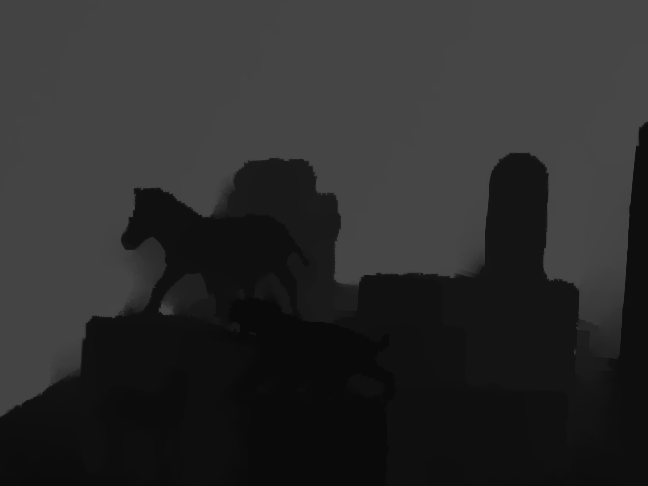
\includegraphics[width=0.9\linewidth]{figure/result_colorized_allregion_noseg.png}
                \caption{\small 使用全局约束但是没有利用语义分割}
                \label{fig:colorize:noseg}
            \end{minipage}
            \begin{minipage}[t]{0.3\linewidth}
                \centering
                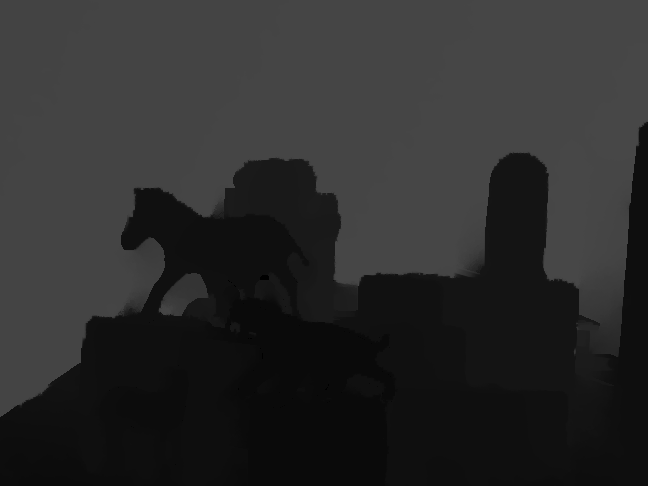
\includegraphics[width=0.9\linewidth]{figure/result_colorized_allregion_seg.png}
                \caption{\small 使用全局约束利用语义分割}
                \label{fig:colorize:seg}
            \end{minipage}
            \begin{minipage}[t]{0.3\linewidth}
                \centering
                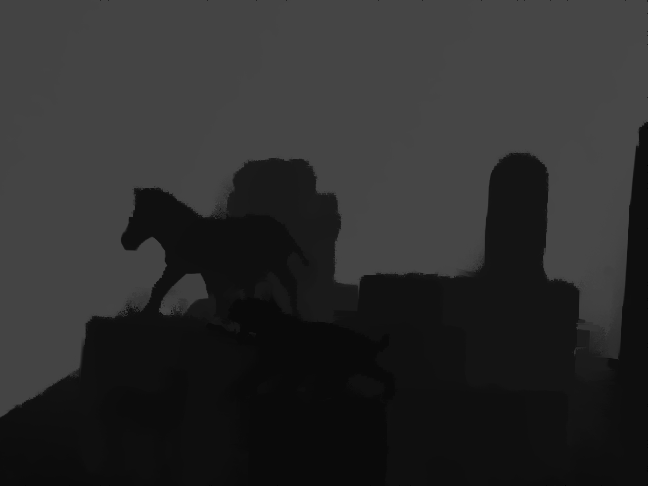
\includegraphics[width=0.9\linewidth]{figure/result_colorized_allergin_minw}
                \caption{\small 利用更大窗口中的最近似策略}
                \label{fig:colorize:minw}
            \end{minipage}
        \end{figure}\par
        \subsection{tgv收敛问题}
        在\myciteup{Ferstl2013}中的算法\ref{alg:TGVL2},可以看成是Chambolle\myciteup{Chambolle2011}提到的$Algorithm 2.$和Pock\myciteup{Diagonal_preconditioning}提到的算法的结合版本。通过引入一个类似学习因子的变量,不断在迭代中缩短优化的步长值。虽然对于初始点比较靠近收敛点的算法,能够起到加快收敛的效果。但是对于我们的使用场景中而言,由于初始点和收敛点
        距离较远,所以反而会减慢收敛速度。对此采取的改进是,将$\tau , \sigma,  \theta $设置成定值。见算法\ref{alg:TGVL2Fixstep}
        \begin{algorithm}
            \caption{pdTGVL2}
            \begin{algorithmic}
                \STATE $\bm{Initialization}$: $Choose \tau_0,\sigma_0 >0, \ with\ \tau_0\sigma_{0}L^2\leq 1, (x^0,y^0)\in X\times Y \ and \ set\ \overline{x}^0=x^0.$
                \STATE $\bm{Caculate\ Tensors}$:$Choose\ \alpha \in[0,2]\ and\ Caculate\ as\ follow:$
                \begin{equation}
                    \begin{aligned}
                        T &= diag(\bm{\tau}) , where\ \bm{\tau} = (\tau_1,...,\tau_n),\tau_j=\frac{1}{\sum_{i=1}^m\left| K_{i,j} \right|^{2-\alpha}},\\
                        \Sigma &= diag(\bm{\sigma}),where\ \bm{\sigma} = (\sigma_1,...,\sigma_m).\sigma_i=\frac{1}{\sum_{j=1}^n\left| K_{i,j} \right|^{\alpha}}\\
                    \end{aligned}
                \end{equation}
                \STATE $\bm{Iterations}(k\geq 0)$:\ $Update\ x^n,y^n,\overline{x}^n\ as\ follows:$
                \begin{equation}
                    \begin{aligned}
                        x^{k+1} &=(I+\tau_k T\partial G)^{-1}(x^k-\tau_k TK^Ty^k ), \\
                        y^{k+1} &=(I+\sigma_k\Sigma\partial F^*)(y^k+\sigma_k \Sigma K\overline{x}^k).\\
                        \theta_k &= \frac{1}{\sqrt {1+2\gamma \tau_k}},\tau_{k+1}=\theta_k\tau_k,\sigma_{k+1}=\frac{\sigma_k}{\tau_n}\\
                        \overline{x}^{k+1} &= x^{k+1}+\theta_k(x^{k+1}-x^k)\\
                    \end{aligned}
                \end{equation}
            \end{algorithmic}
            \label{alg:TGVL2}
        \end{algorithm}
        改善之后的算法效果如图\ref{fig:fasttgv} 所示,可以看到算法收敛速度得到明显改善。
        算法参数为 $iterTimes = 10000, \alpha_w = 17, \alpha_u=5, \lambda = 1e-2,\tau = 1, \sigma = 1, \theta = 1$
        耗时700s(stgv)和1000s(cstgv) ,ITGV迭代5000次,使用的
        参数为$iterTimes = 5000, \alpha_w = 5, \alpha_u=1.2, \lambda = 1e-2,\tau = 1, \sigma = 1, \theta = 1$,耗时为346.905s
        \begin{figure}[htbp]
            \centering
            \subfigure[STGV效果,收敛慢,迭代14730次]{
                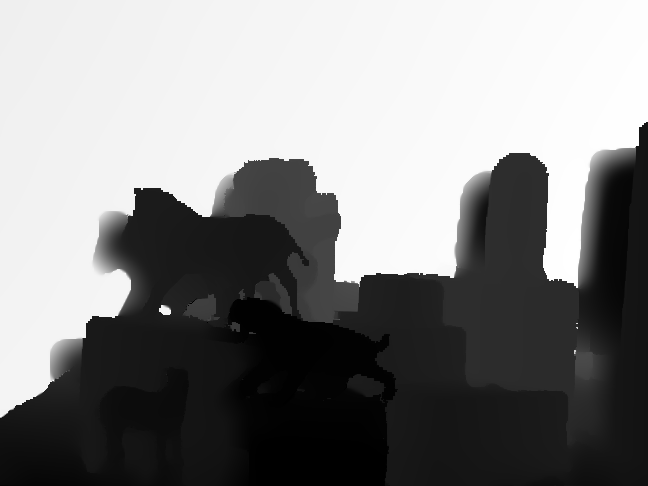
\includegraphics[width=0.45\linewidth]{figure/tgvl2_14730_user_seg}}
            \quad
            \subfigure[STGV效果,收敛快,迭代10000次,耗时700s]{
                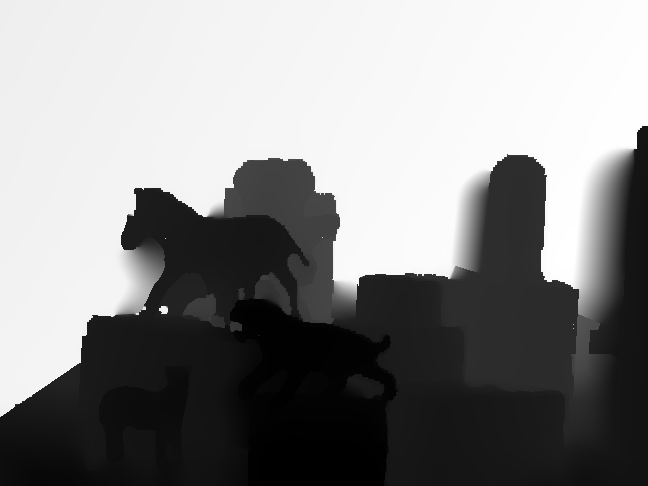
\includegraphics[width=0.45\linewidth]{figure/tgvl2_10000_user_seg}}
            \quad
            \subfigure[CSTGV效果,收敛快,迭代10000次,耗时1000s]{
                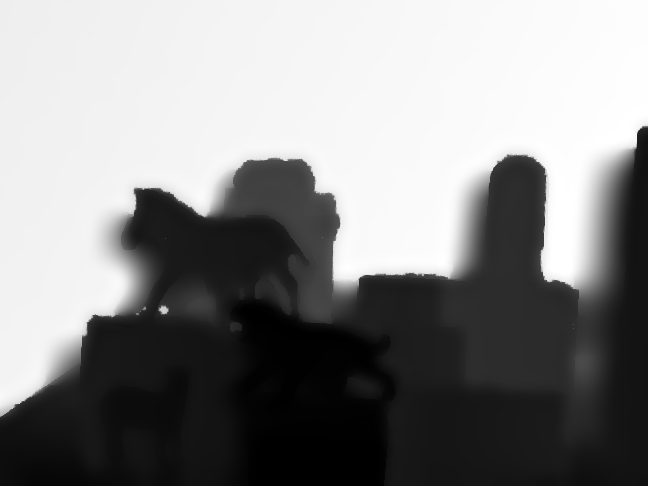
\includegraphics[width=0.45\linewidth]{figure/tgvl2_10000_user_seg_colorize}}
            \quad
            \subfigure[ITGV效果,收敛快,迭代5000次,耗时346.9s]{
                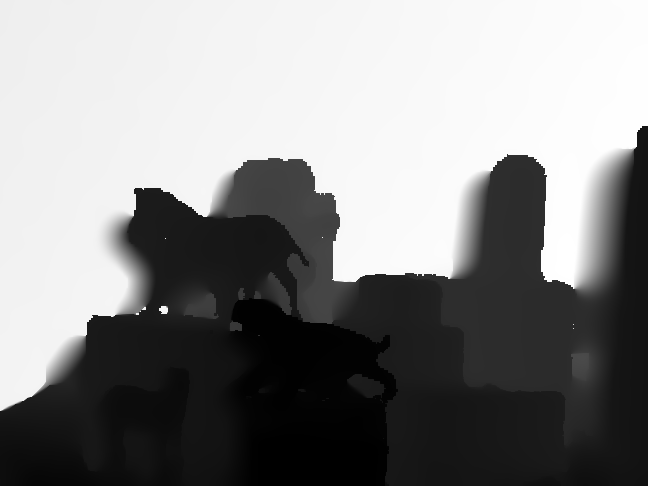
\includegraphics[width=0.45\linewidth]{figure/tgvl2_5000_no_seg}}
            \caption{\small 收敛速度提升后的优化效果}
            \label{fig:fasttgv}
        \end{figure}
        \begin{algorithm}
            \caption{pdTGVL2\_fixStep}
            \begin{algorithmic}
                \STATE $\bm{Initialization}$: $Choose \tau_0,\sigma_0 > 1/ \tau_0, \ \theta = 1, (x^0,y^0)\in X\times Y \ and \ set\ \overline{x}^0=x^0.$
                \STATE $\bm{Caculate\ Tensors}$:$Choose\ \alpha \in[0,2]\ and\ Caculate\ as\ follow:$
                \begin{equation}
                    \begin{aligned}
                        T &= diag(\bm{\tau}) , where\ \bm{\tau} = (\tau_1,...,\tau_n),\tau_j=\frac{1}{\sum_{i=1}^m\left| K_{i,j} \right|^{2-\alpha}},\\
                        \Sigma &= diag(\bm{\sigma}),where\ \bm{\sigma} = (\sigma_1,...,\sigma_m).\sigma_i=\frac{1}{\sum_{j=1}^n\left| K_{i,j} \right|^{\alpha}}\\
                    \end{aligned}
                \end{equation}
                \STATE $\bm{Iterations}(k\geq 0)$:\ $Update\ x^n,y^n,\overline{x}^n\ as\ follows:$
                \begin{equation}
                    \begin{aligned}
                        x^{k+1} &=(I+\tau_0 T\partial G)^{-1}(x^k-\tau_0 TK^Ty^k ), \\
                        y^{k+1} &=(I+\sigma_0\Sigma\partial F^*)(y^k+\sigma_0 \Sigma K\overline{x}^k).\\
                        \overline{x}^{k+1} &= x^{k+1}+\theta(x^{k+1}-x^k)\\
                    \end{aligned}
                \end{equation}
            \end{algorithmic}
            \label{alg:TGVL2Fixstep}
        \end{algorithm}
        实验中发现,TGV算法对正则项f的分布依赖性比较大,当f中存在异常值时,会导致修复效果错误。可以看到,当初始值中移除了错误深度数据之后。
        算法效果得到明显的改善,使用的参数为$iterTimes = 5000, \alpha_w = 5, \alpha_u=1.2, \lambda = 1e-2,\tau = 1, \sigma = 1, \theta = 1$

        \begin{figure}[htbp]
            \centering
            \subfigure[含有错误值的初始图像]{
                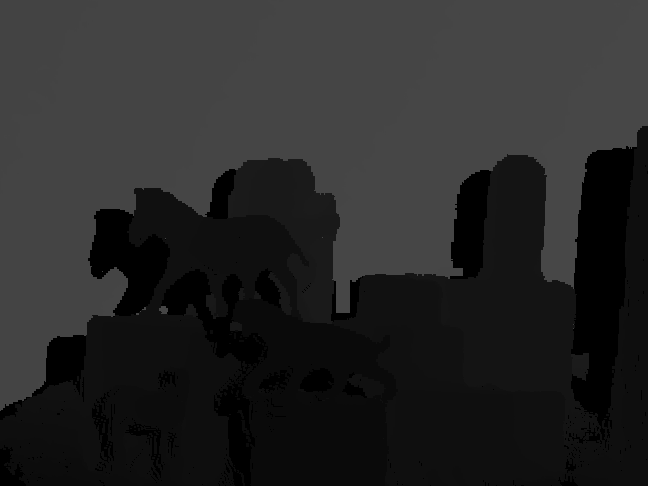
\includegraphics[width=0.45\linewidth]{figure/depthInpaint_withBadPts}}
            \quad
            \subfigure[移除了错误值的初始图像]{
                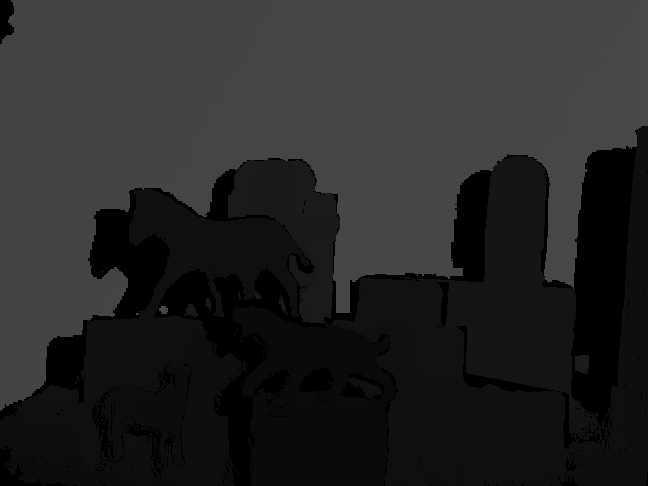
\includegraphics[width=0.45\linewidth]{figure/depthInpaint_removeBadpts}}
            \quad
            \subfigure[用正确初始图像的修复效果,STGV,耗时389.9s]{
                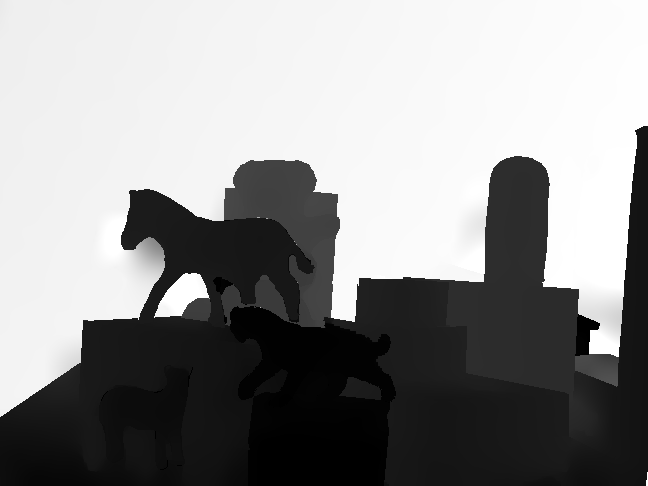
\includegraphics[width=0.45\linewidth]{figure/tgvl2_5000_seg_removeBadPts}}
            \quad
            \subfigure[用正确初始图像的修复效果,CSTGV,耗时577s]{
                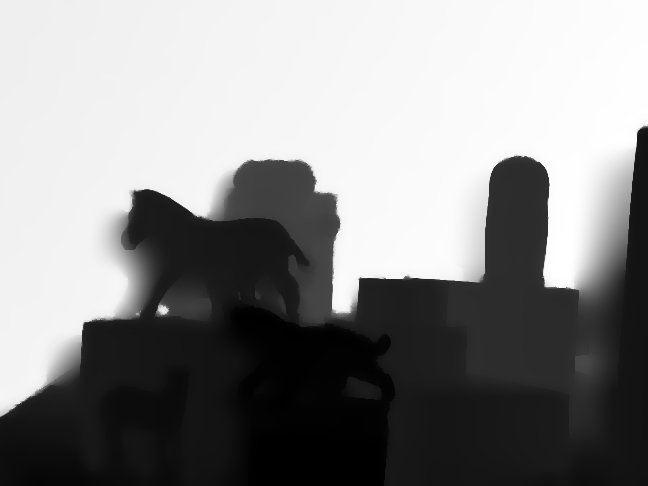
\includegraphics[width=0.45\linewidth]{figure/colorizeFPrecodition_5000_removeBadPts}}
            \caption{\small 初始值对TGV效果影响}
            \label{fig:fasttgv}
        \end{figure}\par

        使用循环边界测试了一下tgv的收敛效果。发现循环边界会引入异常,见图\ref{fig:badEdgeLoopD},分析可能的原因是,因为用了循环边界差分,
        在第m行的$\nabla_y$的计算中引入了第0行的数据,也就是第0行的深度值会影响最后一行的深度补偿效果。
        \begin{figure}[htbp]
            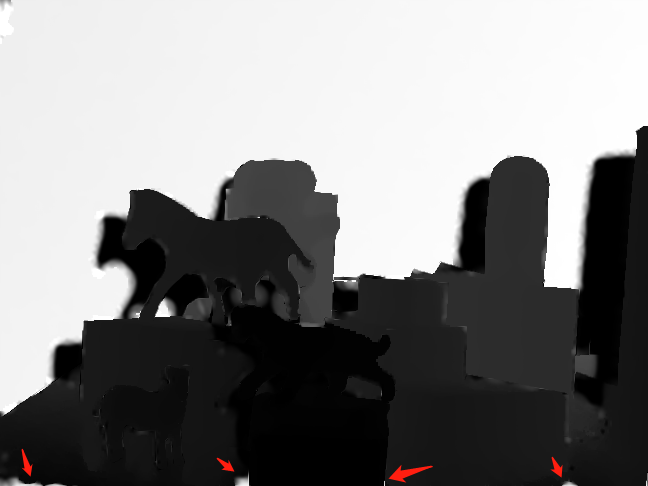
\includegraphics[width=0.9\linewidth]{figure/badEdgeD}
            \caption{\small 循环边界导致数据异常}
            \label{fig:badEdgeLoopD}
        \end{figure}
        \section{单目深度测算}
        \subsection{色差dfd}
        利用透镜的对不同颜色的对焦参数(焦距)不同,可以利用单张图片进行深度信息解算\myciteup{buat2020active}\myciteup{ishihara2021depth}。
        色差信息的使用带来的好处是只用一张图片就可以解决传统dfd深度解算的二义性,也即只通过一张图片,仅能估计处模糊半径,但是模糊半径可能是对焦像平面在
        传感器靶面之前或者之后的两种可能位置造成的。也就是可能的深度解有两个。而色差信息,由于不同波长的光的焦距不一样,其成像的模糊半径也不一样,一张图片可以
        获取多种光谱的不同的模糊半径,因此能够消除深度解算的二义性。
        \begin{figure}[htbp]
            \subfigure[模糊形成示意]{
            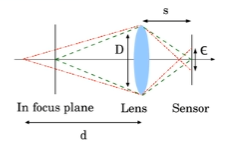
\includegraphics[width=0.45\linewidth]{figure/deblurOPtics}
            }
            \quad
            \subfigure[单张DFD解算二义性]{
                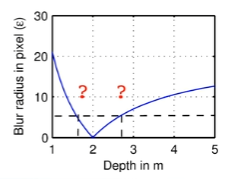
\includegraphics[width=0.45\linewidth]{figure/DFD-ambiguity}
            }
            \quad
            \subfigure[多光谱DFD示意]{
            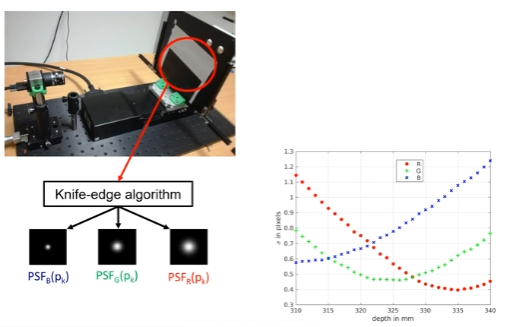
\includegraphics[width=0.8\linewidth]{figure/active-chromatic-DFD}
            }
            \caption{\small 色差DFD\myciteup{buat2020active}}
            \label{fig:activechromatic}
        \end{figure}
        受其启发,是否可以利用像散进行DFD计算。也即将液晶透镜水平和垂直的光焦度设置成不同的值,形成椭圆形透镜,由于像散的图像在不同的深度范围具有不同的长轴和短轴,因此
        可以消除二义性。
        \begin{figure}[htbp]
            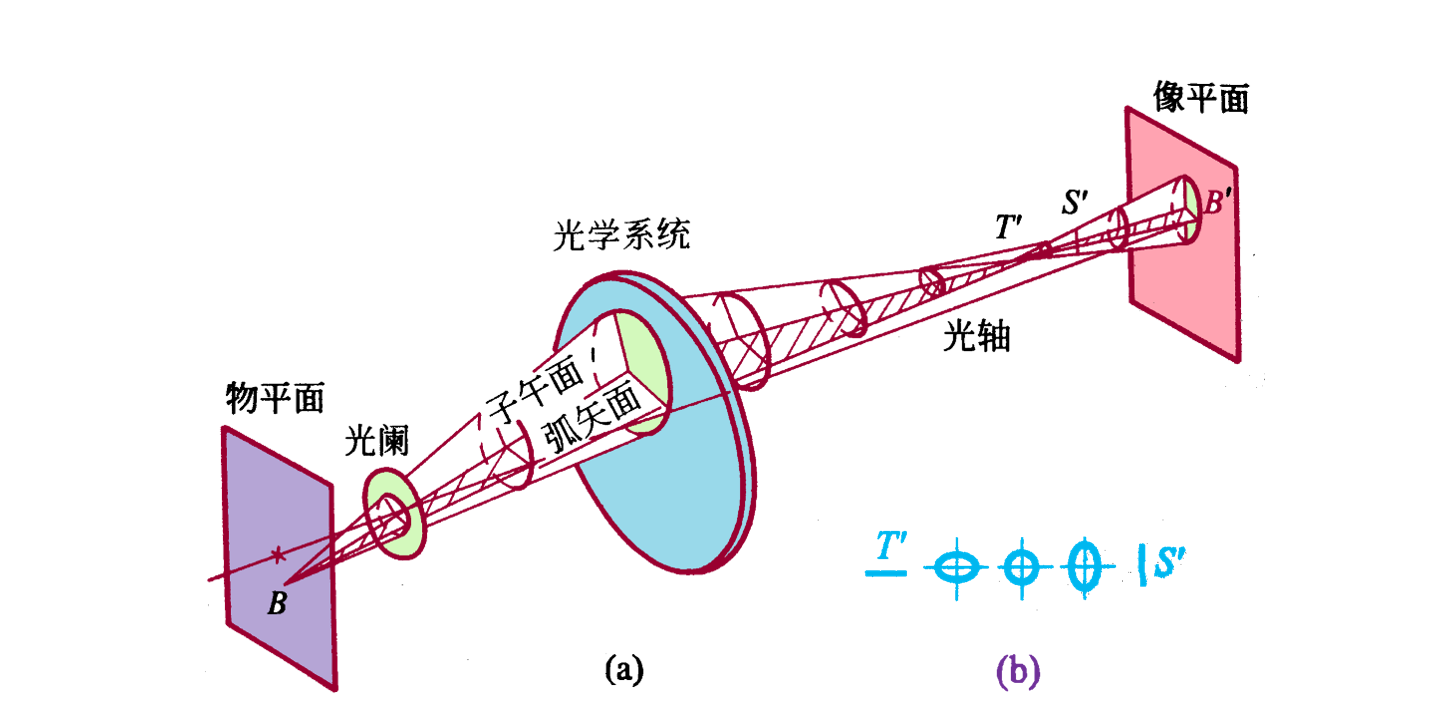
\includegraphics[width=0.9\linewidth]{figure/Astigmatism}
            \caption{\small 像散示意图\myciteup{yeOptics}}
            \label{fig:astigmatism}
        \end{figure}
        利用Levin\myciteup{levin2007image}提出的KL散度模型来测算椭圆形的模糊光斑在相近距离的区分度。
        \begin{equation}
            \begin{aligned}
            D_{KL}(P_{k1},P_{k2}) &= \sum\limits{v,w}(\frac{\sigma_{k1}(v,w)}{\sigma_{k2}(v,w)} - \log (\frac{\sigma_{k1}(v,w)}{\sigma_{k2}(v,w)}))\\
            \sigma(v,w) &= \left | F_k(v,w) \right |^2(\alpha\left | G_x(v,w) \right |^2 + \alpha \left | G_y(v,w) \right |^2)^{-1} + \eta^2
            \end{aligned}
        \end{equation}
        其中$F_k(v,w)$为PSF的傅里叶变换,$G_x(v,w),G_y(v,w)$为水平和垂直差分算子的傅里叶变换。$\eta$为噪声的方差。椭圆透镜的KL散度见图\ref{fig:EclipseKl}
        \begin{figure}[htbp]
            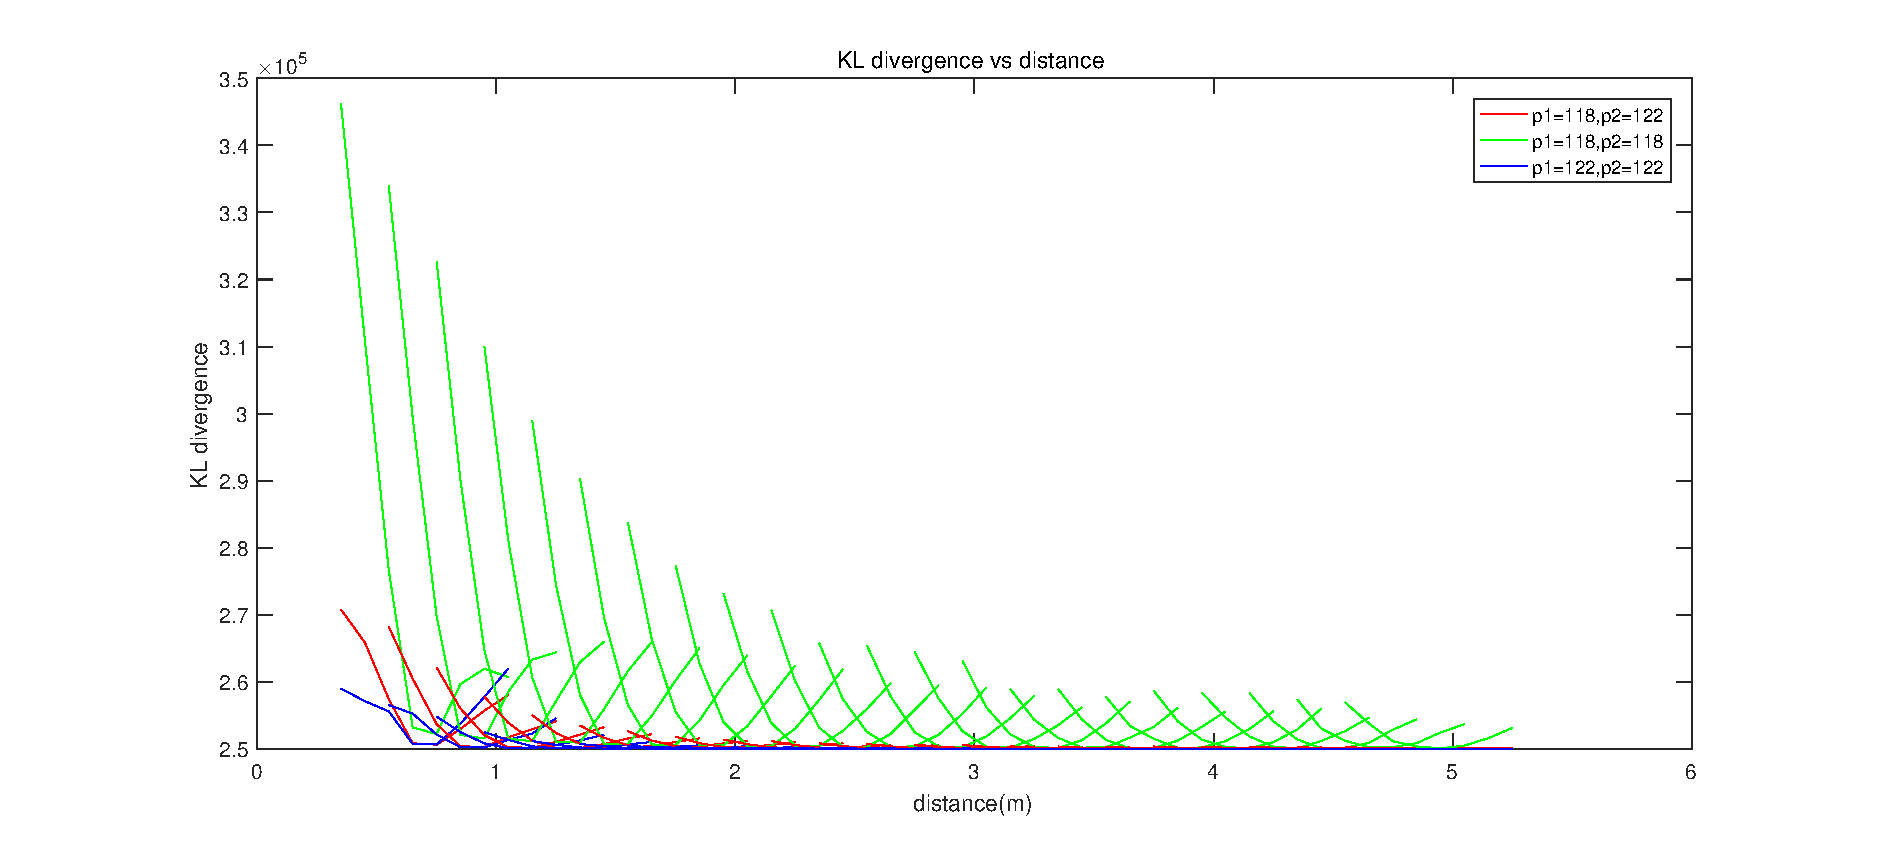
\includegraphics[width=0.9\linewidth]{figure/kldivergence_vs_distance}
            \caption{\small 椭圆透镜的KL散度}
            \label{fig:EclipseKl}
        \end{figure}
        \section{接下来的工作}
        \begin{itemize}
            \item 结合文献\myciteup{rajagopalan1999mrf}和文献\myciteup{saxena2005learning},编写dfd算法,考虑结合使用多尺度信息和其他的结构信息;
            \item 进一步实验验证单张图进行DFD的可能性
        \end{itemize}


    \bibliography{main}
    \bibliographystyle{plain}
    \end{sloppypar}

\end{document}
